\documentclass[10pt]{beamer}\usepackage[]{graphicx}\usepackage[]{color}
%% maxwidth is the original width if it is less than linewidth
%% otherwise use linewidth (to make sure the graphics do not exceed the margin)
\makeatletter
\def\maxwidth{ %
  \ifdim\Gin@nat@width>\linewidth
    \linewidth
  \else
    \Gin@nat@width
  \fi
}
\makeatother

\definecolor{fgcolor}{rgb}{0.345, 0.345, 0.345}
\newcommand{\hlnum}[1]{\textcolor[rgb]{0.686,0.059,0.569}{#1}}%
\newcommand{\hlstr}[1]{\textcolor[rgb]{0.192,0.494,0.8}{#1}}%
\newcommand{\hlcom}[1]{\textcolor[rgb]{0.678,0.584,0.686}{\textit{#1}}}%
\newcommand{\hlopt}[1]{\textcolor[rgb]{0,0,0}{#1}}%
\newcommand{\hlstd}[1]{\textcolor[rgb]{0.345,0.345,0.345}{#1}}%
\newcommand{\hlkwa}[1]{\textcolor[rgb]{0.161,0.373,0.58}{\textbf{#1}}}%
\newcommand{\hlkwb}[1]{\textcolor[rgb]{0.69,0.353,0.396}{#1}}%
\newcommand{\hlkwc}[1]{\textcolor[rgb]{0.333,0.667,0.333}{#1}}%
\newcommand{\hlkwd}[1]{\textcolor[rgb]{0.737,0.353,0.396}{\textbf{#1}}}%
\let\hlipl\hlkwb

\usepackage{framed}
\makeatletter
\newenvironment{kframe}{%
 \def\at@end@of@kframe{}%
 \ifinner\ifhmode%
  \def\at@end@of@kframe{\end{minipage}}%
  \begin{minipage}{\columnwidth}%
 \fi\fi%
 \def\FrameCommand##1{\hskip\@totalleftmargin \hskip-\fboxsep
 \colorbox{shadecolor}{##1}\hskip-\fboxsep
     % There is no \\@totalrightmargin, so:
     \hskip-\linewidth \hskip-\@totalleftmargin \hskip\columnwidth}%
 \MakeFramed {\advance\hsize-\width
   \@totalleftmargin\z@ \linewidth\hsize
   \@setminipage}}%
 {\par\unskip\endMakeFramed%
 \at@end@of@kframe}
\makeatother

\definecolor{shadecolor}{rgb}{.97, .97, .97}
\definecolor{messagecolor}{rgb}{0, 0, 0}
\definecolor{warningcolor}{rgb}{1, 0, 1}
\definecolor{errorcolor}{rgb}{1, 0, 0}
\newenvironment{knitrout}{}{} % an empty environment to be redefined in TeX

\usepackage{alltt}

\usepackage{graphicx, color}
\usepackage{alltt}
\usepackage{booktabs, calc, rotating}
\usepackage[round]{natbib}
\usepackage{pdfpages, subfigure}
\usepackage{multicol}
\usepackage{amsmath, amsbsy, amssymb, amsthm, graphicx}
\usepackage[english]{babel}
\usepackage{xkeyval} 
\usepackage{xfrac}
\usepackage{multicol}
\usepackage[normalem]{ulem}
\usepackage{multirow, fancyvrb} 
\usepackage{tikz, geometry, tkz-graph, xcolor}
\usepackage{listings}

\let\oldemptyset\emptyset
\let\emptyset\varnothing

\renewenvironment{knitrout}{\setlength{\topsep}{-.2mm}}{}

\usetikzlibrary{arrows,positioning} 
\tikzset{
  % Define standard arrow tip
  >=stealth',
  % Define style for boxes
  punkt/.style={
    rectangle,
    rounded corners,
    draw=black, very thick,
    text width=6.5em,
    minimum height=2em,
    text centered},
  % Define arrow style
  pil/.style={
    ->,
    thick,
    shorten <=2pt,
    shorten >=2pt,}
}
\usetikzlibrary{trees}
% Set the overall layout of the tree
\tikzstyle{level 1}=[level distance=2.5cm, sibling distance=4cm] 
\tikzstyle{level 2}=[level distance=2.5cm, sibling distance=2.5cm]
\tikzstyle{level 3}=[level distance=2.5cm, sibling distance=1cm]

% Define styles for bags and leafs
\tikzstyle{bag} = [text width=4em, text centered]
\tikzstyle{end} = [circle, minimum width=3pt,fill, inner sep=0pt]
\tikzstyle{openend} = [circle, minimum width=3pt, inner sep=0pt]

\hypersetup{colorlinks, citecolor=blue, linkcolor=., menucolor=white, filecolor=blue, anchorcolor=yellow}

\usetikzlibrary{arrows,positioning} 
\tikzset{
  % Define standard arrow tip
  >=stealth',
  % Define style for boxes
  punkt/.style={rectangle, rounded corners, draw=black, very thick, text width=6.5em, 
    minimum height=2em, text centered},
  % Define arrow style
  pil/.style={ ->, thick, shorten <=2pt, shorten >=2pt,}}

\graphicspath{{figure/}}

\newcommand{\cov}{\mathrm{cov}}
\newcommand{\dif}{\mathrm{d}}
\newcommand{\bigbrk}{\vspace*{2in}}
\newcommand{\smallbrk}{\vspace*{.1in}}
\newcommand{\midbrk}{\vspace*{1in}}
\newcommand{\red}[1]{{\color{red}#1}}
\newcommand{\empr}[1]{{\emph{\color{red}#1}}}
\newcommand{\blue}[1]{{\color{blue}#1}}
\newcommand{\green}[1]{{\color{green}#1}}
\newcommand{\pkg}[1]{{\textbf{\texttt{#1}}}}
\newcommand{\code}[1]{{\texttt{#1}}}
\newcommand{\calc}[1]{{\fbox{\mbox{#1}}}}
\newcommand{\Var}{\mathrm{Var}}
\newcommand{\var}{\mathrm{var}}
\newcommand{\E}{\mathrm{E}}
\newcommand{\I}{\mathrm{I}}
\newcommand{\p}{\mathrm{P}}
\newcommand{\Skm}{\hat{S}_{\scriptsize{KM}}}
\newcommand{\Sna}{\hat{S}_{\scriptsize{NA}}}
\newcommand{\V}{\mathrm{V}}
\newcommand{\R}{\texttt{R}}
\newcommand{\Cov}{\mathrm{Cov}}

\mode<presentation> {
  \usetheme{UTD}
  \usecolortheme[RGB={200,0,0}]{structure}
  \setbeamercovered{transparent}
}

\usepackage[latin1]{inputenc}
\usepackage{times}
\usepackage[T1]{fontenc}

\DeclareSymbolFont{extraup}{U}{zavm}{m}{n}
\DeclareMathSymbol{\varheart}{\mathalpha}{extraup}{86}
\DeclareMathSymbol{\vardiamond}{\mathalpha}{extraup}{87}

\newcommand*{\mybox}[1]{\framebox{#1}}

\title[STAT 6390]{STAT 6390: Analysis of Survival Data\\
  \small{Textbook coverage: Chapter 2}\\}
\author[Steven Chiou]{Steven Chiou}
\institute[UTD]{Department of Mathematical Sciences, \\ University of Texas at Dallas}
\date{}

% UTD logo on top right corner
% \usepackage[absolute, overlay]{textpos}
% \addtobeamertemplate{frametitle}{}{%
% \begin{textblock*}{100cm}(.94\textwidth, 0.6cm)
%   \includegraphics[trim = 1.8cm .9cm 1.8cm .92cm, clip, scale = .28, keepaspectratio]{UTDlogo}
% \end{textblock*}}
\IfFileExists{upquote.sty}{\usepackage{upquote}}{}
\begin{document}

\begin{frame}[fragile]
  \titlepage

\end{frame}

\setbeamercolor*{item}{fg=red}
\bgroup
\usebackgroundtemplate{%
  \tikz[overlay,remember picture] \node[opacity=0.05, at=(current page.center)] {
    
\includegraphics[height=\paperheight,width=\paperwidth]{UTDbg}};}

\section{Survivor, hazard and cumulative hazard functions}
\begin{frame}[fragile]
  \frametitle{Survivor, hazard and cumulative hazard functions}
  \begin{itemize}
  \item Suppose the actual (uncensored, untruncated) survival time of an individual is $t$
    and can be regarded as the observed value of a variable, $T$.
  \item We assume the support of $T$ is non-negative or $(0, \infty)$.
  \item We call $T$ the \emph{random variable} associated with the survival time, 
    and we define $T$ has a cumulative distribution function given by
    $F(t) = \p(T \le t)$.
  \item The survival function of $T$ is then defined as $$S(t) = 1 - \p(T\le t) = 1 - F(t).$$
  \item Why are we more interested in $S(t)$?
  \end{itemize}


\end{frame}

\begin{frame}
  \frametitle{Survivor, hazard and cumulative hazard functions}
  \begin{itemize}
    \item The \empr{hazard function} is widely used to survival analysis. 
    \item The hazard function $h(t)$ is defined below
      \begin{equation}
        h(t) = \lim_{\delta\to0}\frac{\p(t\le T < t + \delta|T\ge t)}{\delta}.
        \label{eq:haz}
      \end{equation}
    \item $\p(t\le T< t + \delta|T\ge t)$ is a conditional probability.
      %the probability $T$ lies between $t$ and $t + \delta$ \emph{condition on} $T \ge t$.
    \item The conditional probability is then expressed as a probability per nit time by dividing by the time interval, $\delta$, to give a \emph{rate}.
    \item The function $h(t)$ is also referred to as the \empr{hazard rate}, the \empr{instantaneous death rate}, 
      the \empr{intensity rate}, or the \empr{force of mortality}.
    \item Event rate at time $t$, conditional on the event not having occurred before $t$.
    \end{itemize}
\end{frame}

\begin{frame}
  \frametitle{Survivor, hazard and cumulative hazard functions}
  \begin{itemize}
    \item In terms of probability, if $t$ is measured in days, $h(t)$ is the approximate probability that an individual, 
      who is \emph{at risk} of the event occurring at the start of day $t$, experiences the event during that day.
      \begin{itemize}
      \item In this case $\delta = 1$.
      \item $\lim_{\delta \to0}$ can be thought of as changing the unit from days to hours, minutes, seconds, milliseconds...
      \end{itemize}
    \item If the event of interest is not death, $h(t)$ can also be regarded as the \emph{expected number of events}
      experienced by an individual in unit time, given that the event has not occurred before then. 
      \begin{itemize}
        \item Think of $\E\{\I(\cdot)\} = \p(\cdot)$.
        \item The part ``given that the event...'' might be ignored if events follow the Poisson process.
        \end{itemize}
      \end{itemize}
\end{frame}

\begin{frame}
  \frametitle{Survivor, hazard and cumulative hazard functions}
  \begin{itemize}
    \item The definition in~\eqref{eq:haz} leads to some useful relationships between survivor and hazard functions:
      \begin{equation*}
        \hspace{-.5cm}
        (1) = \lim_{\delta\to0}\frac{\p(t\le T < t + \delta)}{\delta\cdot\p(T < t)} = 
        \lim_{\delta\to0}\frac{F(t + \delta) - F(t)}{\delta} \cdot \frac{1}{\p(T < t)} =
        \frac{\dif F(t)}{\dif t}\cdot \frac{1}{S(t)}.
      \end{equation*}
    \item $h(t)$ is approximately the probability that an individual experiences an event at this instant ($t$)
      given that he/she is risk free up to $t$.
    \item If $T$ is a continuous random variable, then we have 
      \begin{equation}
        h(t) = \frac{f(t)}{S(t)}.
        \label{eq:haz2}
      \end{equation}
    \item This shows that from any one of the three functions, $f(t)$, $S(t)$, and $h(t)$, 
      the other two can be determined. 
  \end{itemize}
\end{frame}

\begin{frame}
  \frametitle{Survivor, hazard and cumulative hazard functions}
  \begin{itemize}
    \item Equation~\eqref{eq:haz2} also implies
      $$h(t) = -\frac{\dif}{\dif t}\left\{ \log S(t)\right\} \mbox{ and } S(t) = e^{-H(t)},$$
      where $H(t) = \int_0^th(u)\,\dif u$ is the \empr{cumulative hazard function}.
    \item Similarly, the cumulative hazard function can also be obtained from 
      $$H(t) = -\log S(t).$$
    \item The cumulative hazard function is the cumulative risk of an event occurring by time $t$.
    \item If the event is death, then $H(t)$ summarizes the risk of death up to time $t$, given that death has not occurred by $t$.
    \item If the event is not death, $H(t)$ can be interpreted as the expected number of events that occur in the interval $(0, t)$.
  \end{itemize}
\end{frame}


\begin{frame}
  \frametitle{Survivor, hazard and cumulative hazard functions}
  \begin{itemize}
    \item It is possible for $H(t) > 1$, $h(t) > 1$, or $f(t) > 1$.
    \item Like $F(t)$, $S(t)$ is bounded in $[0, 1]$.
    \item $F(t)$ and $H(t)$ is non-decreasing; $S(t)$ is non-increasing.
    \item $h(t)$ can go up and down.
    \item For example, suppose $T\sim\exp(\lambda)$, where $\lambda$ is the rate. Then
      \begin{itemize}
      \item $S(t) = e^{\lambda t}$.
      \item $h(t) = \lambda$.
      \item $H(t) = \lambda t$.
  \end{itemize}
\end{itemize}
\end{frame}

\section{Estimating $S(t)$}

\begin{frame}
  \frametitle{Empirical survivor function}
  \begin{itemize}
  \item The $S(t)$ can be estimated non-parametrically with the \empr{product limit} estimator, 
    which is also known as the \empr{Kaplan-Meier} estimator.
  \item We first assume there is a single sample of survival times, 
    and none of these are censored. 
  \item In this case, the survivor probability at $t$, $S(t)$, is defined as 
    \begin{equation}
      \hat S_e(t) = \frac{\mbox{\# individuals with survival times} \ge t}{\mbox{\# individuals in the data set}}.
        \label{eq:empS}
    \end{equation}
  \item Equation~\eqref{eq:empS} is called \empr{empirical survivor function}. 
  \item Similar $\hat F_e(t) = 1 - \hat S_e(t)$ is called the \empr{empirical cumulative distribution function}.
    \end{itemize}
\end{frame}

\begin{frame}[fragile]
  \frametitle{Empirical survivor function}
  \begin{itemize}
  \item We illustrate with the first 10 uncensored subjects in the \texttt{whas100} data.
  \item Make sure \pkg{tidyverse} package and \code{whas100} are properly loaded*.

\begin{knitrout}\scriptsize
\definecolor{shadecolor}{rgb}{0.969, 0.969, 0.969}\color{fgcolor}\begin{kframe}
\begin{alltt}
\hlstd{> }\hlstd{whas10} \hlkwb{<-} \hlstd{whas100} \hlopt \hlkwd{filter}\hlstd{(fstat} \hlopt{>} \hlnum{0}\hlstd{)} \hlopt \hlkwd{filter}\hlstd{(}\hlkwd{row_number}\hlstd{()} \hlopt{<=} \hlnum{10}\hlstd{)}
\hlstd{> }\hlstd{whas10}
\end{alltt}
\begin{verbatim}
# A tibble: 10 x 9
      id admitdate  foldate      los lenfol fstat   age gender   bmi
   <int> <fct>      <fct>      <int>  <int> <int> <int>  <int> <dbl>
 1     1 3/13/1995  3/19/1995      4      6     1    65      0  31.4
 2     2 1/14/1995  1/23/1996      5    374     1    88      1  22.7
 3     3 2/17/1995  10/4/2001      5   2421     1    77      0  27.9
 4     4 4/7/1995   7/14/1995      9     98     1    81      1  21.5
 5     5 2/9/1995   5/29/1998      4   1205     1    78      0  30.7
 6     6 1/16/1995  9/11/2000      7   2065     1    82      1  26.5
 7     7 1/17/1995  10/15/1997     3   1002     1    66      1  35.7
 8     8 11/15/1994 11/24/2000    56   2201     1    81      1  28.3
 9     9 8/18/1995  2/23/1996      5    189     1    76      0  27.1
10    12 5/26/1995  9/29/1996     11    492     1    83      0  24.7
\end{verbatim}
\end{kframe}
\end{knitrout}
\end{itemize}
\hfill\tiny* see note 1 for details.
\end{frame}

\begin{frame}[fragile]
  \frametitle{Empirical survivor function}
  \begin{itemize}
  \item The empirical estimates can be easily computed with \code{ecdf}.
  \end{itemize}
\begin{knitrout}\scriptsize
\definecolor{shadecolor}{rgb}{0.969, 0.969, 0.969}\color{fgcolor}\begin{kframe}
\begin{alltt}
\hlstd{> }\hlstd{whas10} \hlkwb{<-} \hlstd{whas10} \hlopt \hlkwd{mutate}\hlstd{(}\hlkwc{surv} \hlstd{=} \hlnum{1} \hlopt{-} \hlkwd{ecdf}\hlstd{(lenfol)(lenfol))}
\hlstd{> }\hlstd{whas10}
\end{alltt}
\begin{verbatim}
# A tibble: 10 x 10
      id admitdate  foldate      los lenfol fstat   age gender   bmi  surv
   <int> <fct>      <fct>      <int>  <int> <int> <int>  <int> <dbl> <dbl>
 1     1 3/13/1995  3/19/1995      4      6     1    65      0  31.4 0.9  
 2     2 1/14/1995  1/23/1996      5    374     1    88      1  22.7 0.6  
 3     3 2/17/1995  10/4/2001      5   2421     1    77      0  27.9 0    
 4     4 4/7/1995   7/14/1995      9     98     1    81      1  21.5 0.8  
 5     5 2/9/1995   5/29/1998      4   1205     1    78      0  30.7 0.3  
 6     6 1/16/1995  9/11/2000      7   2065     1    82      1  26.5 0.200
 7     7 1/17/1995  10/15/1997     3   1002     1    66      1  35.7 0.4  
 8     8 11/15/1994 11/24/2000    56   2201     1    81      1  28.3 0.100
 9     9 8/18/1995  2/23/1996      5    189     1    76      0  27.1 0.7  
10    12 5/26/1995  9/29/1996     11    492     1    83      0  24.7 0.5  
\end{verbatim}
\end{kframe}
\end{knitrout}
\end{frame}

\begin{frame}[fragile]
  \frametitle{Empirical survivor function}
  \begin{itemize}
  \item The empirical survivor function is a non-increasing step function.
  \end{itemize}
\begin{knitrout}\scriptsize
\definecolor{shadecolor}{rgb}{0.969, 0.969, 0.969}\color{fgcolor}\begin{kframe}
\begin{alltt}
\hlstd{> }\hlstd{whas20} \hlopt \hlkwd{ggplot}\hlstd{(}\hlkwd{aes}\hlstd{(lenfol, surv))} \hlopt{+} \hlkwd{geom_step}\hlstd{(}\hlkwc{size} \hlstd{=} \hlnum{1.2}\hlstd{)}
\end{alltt}
\end{kframe}
\end{knitrout}
  \begin{center}
    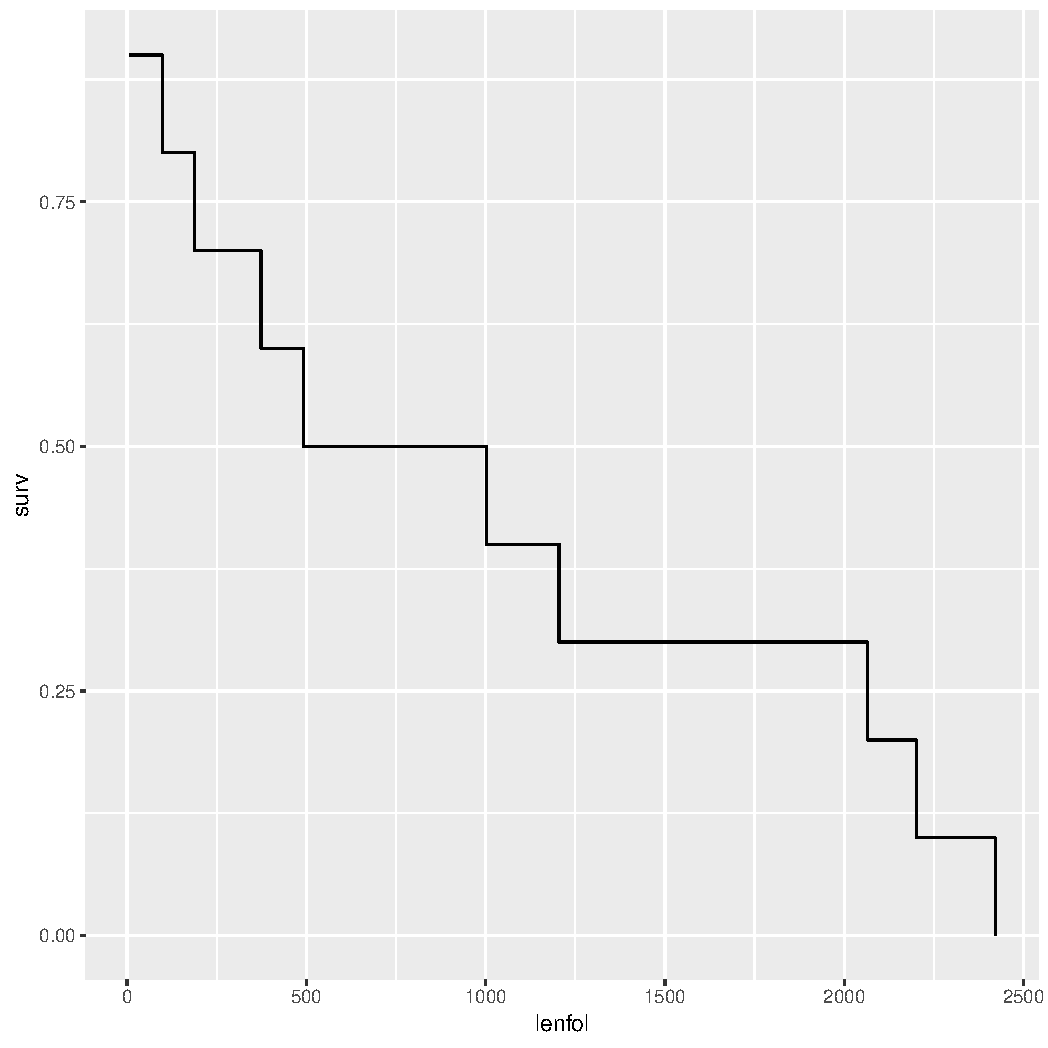
\includegraphics[scale = .3]{whas10-ecdf}
  \end{center}
  \begin{itemize}
  \item The $\hat S_e(t)$ is 1 at $t = 0$ and 0 at the final death time. %, $\max(t)$.
  \item The $\hat S_e(t)$ is assumed to be constant between adjacent death times.
  \end{itemize}
\end{frame}

\begin{frame}[fragile]
  \frametitle{Empirical survivor function}
  \begin{itemize}
  \item Putting everything together, we could plot the empirical survival curve for all the uncensored subjects in \code{whas100}:
  \end{itemize}
\begin{knitrout}\scriptsize
\definecolor{shadecolor}{rgb}{0.969, 0.969, 0.969}\color{fgcolor}\begin{kframe}
\begin{alltt}
\hlstd{> }\hlstd{whas100} \hlopt \hlkwd{filter}\hlstd{(fstat} \hlopt{>} \hlnum{0}\hlstd{)} \hlopt \hlkwd{mutate}\hlstd{(}\hlkwc{surv} \hlstd{=} \hlnum{1} \hlopt{-} \hlkwd{ecdf}\hlstd{(lenfol)(lenfol))} \hlopt
\hlstd{+ }    \hlkwd{ggplot}\hlstd{(}\hlkwd{aes}\hlstd{(lenfol, surv))} \hlopt{+} \hlkwd{geom_step}\hlstd{()} \hlopt{+} \hlkwd{geom_smooth}\hlstd{()}
\end{alltt}
\end{kframe}
\end{knitrout}
  \begin{center}
    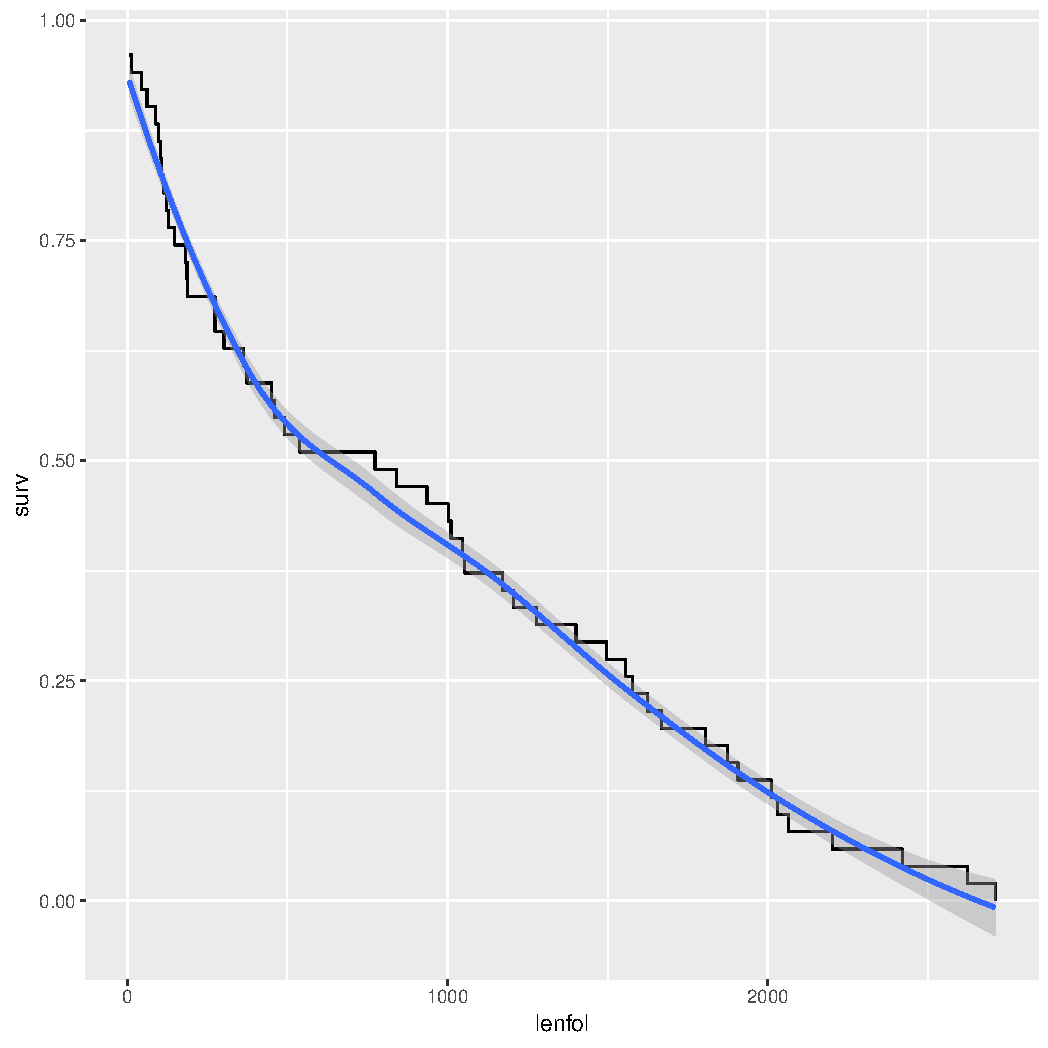
\includegraphics[scale = .3]{whas100-ecdf}
  \end{center} \vspace{-.3cm}
  \begin{itemize}
  \item The pipeline between \code{ggplot} is ``$+$'' instead of ``\code{\%>\%}''.
  \end{itemize}
\end{frame}


\begin{frame}[fragile]
  \frametitle{Kaplan-Meier estiamtor}
  \begin{itemize}
  \item With censoring, the same idea can be applied with proper adjustment.
  \item Kaplan-Meier estimator is the default estimator used by many packages. 
  \item The basic idea is to decompose $\p(T > t)$ by conditioning on prior times.
  \item Suppose a sample size of $n$, $\p(T>t)$ can be decomposed as
    {\scriptsize
    \begin{equation*}
      \Skm(t) \equiv  \p(T > t) = 
      \p(T > t_{(0)}) \cdot \p(T > t_{(1)} | T > t_{(0)}) \cdot \p(T > t_{(2)} | T > t_{(1)}) 
      \cdot\ldots\cdot \p(T > t | T > t_{(i)}),
    \end{equation*}}
    for a series of time intervals $0 \equiv t_{(0)} < t_{(1)} < \ldots < t_{(i)} < t$ for some $i\le n$.
  \item In general, the series $\{t_{(1)}, \ldots, t_{(m)}\}$ 
    denotes the $m$ ordered death times.
  \end{itemize}
\end{frame}

\begin{frame}
  \frametitle{Kaplan-Meier estiamtor}
  Suppose we want $\p(T > 800)$ among the first 20 patients in \texttt{whas1000}.
  \begin{columns}
    \column{0.45\textwidth}
    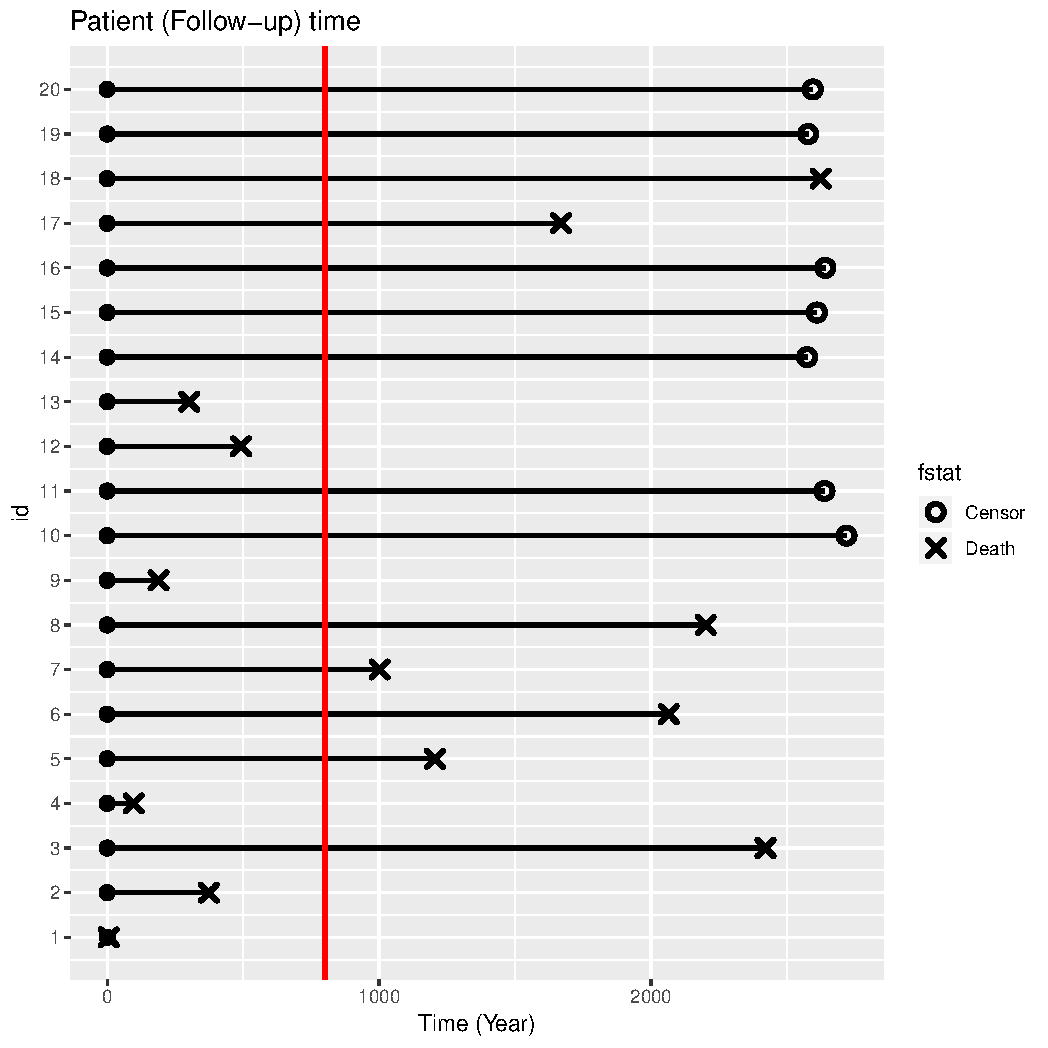
\includegraphics[scale = .3]{tab1-1-4}
    \column{0.55\textwidth}
    \begin{itemize}
    \item There are 6 events before $t = 800$.
    \item The events occured at 
      {\scriptsize
      \begin{tabular}{lllllll}
        $t_{(0)}$ & $t_{(1)}$ & $t_{(2)}$ & $t_{(3)}$ & $t_{(4)}$ & $t_{(5)}$ & $t_{(6)}$ \\
        \midrule
        0 & 6 & 98 & 189 & 302 & 374 & 492 \\
      \end{tabular}}
    \end{itemize}
  \end{columns}
  \vspace{-.3cm}
  {\scriptsize
  \begin{align*}
    \Skm(800) &= \p(T > 800) =\\
    &= \p(T > 0) \times \p(T > 6|T > 0) \times \p(T > 98|T > 6) \times
    \ldots\times \p(T > 492|T > 374) \\
    &=1 \times \frac{19}{20} \times \frac{18}{19} \times \frac{17}{18} \times \frac{16}{17} \times \frac{15}{16} \times 
    \frac{14}{15} = \frac{14}{20} = 70\%
  \end{align*}
  }
  Why does $\Skm(800) = \hat S_e(800)$ here?
\end{frame}

\begin{frame}[fragile]
  \frametitle{Kaplan-Meier estimator}
  \begin{itemize}
  \item The Kaplan-Meier estimator can be obtained with the \code{survfit} function.
    % from \pkg{survival}.
\begin{knitrout}\scriptsize
\definecolor{shadecolor}{rgb}{0.969, 0.969, 0.969}\color{fgcolor}\begin{kframe}
\begin{alltt}
\hlstd{> }\hlkwd{library}\hlstd{(survival)}
\hlstd{> }\hlstd{km} \hlkwb{<-} \hlkwd{survfit}\hlstd{(}\hlkwd{Surv}\hlstd{(lenfol, fstat)} \hlopt{~} \hlnum{1}\hlstd{,} \hlkwc{data} \hlstd{= whas100,} \hlkwc{subset} \hlstd{= id} \hlopt{<=} \hlnum{20}\hlstd{)}
\hlstd{> }\hlkwd{summary}\hlstd{(km)}
\end{alltt}
\begin{verbatim}
Call: survfit(formula = Surv(lenfol, fstat) ~ 1, data = whas100, subset = id <= 
    20)

 time n.risk n.event survival std.err lower 95% CI upper 95% CI
    6     20       1     0.95  0.0487        0.859        1.000
   98     19       1     0.90  0.0671        0.778        1.000
  189     18       1     0.85  0.0798        0.707        1.000
  302     17       1     0.80  0.0894        0.643        0.996
  374     16       1     0.75  0.0968        0.582        0.966
  492     15       1     0.70  0.1025        0.525        0.933
 1002     14       1     0.65  0.1067        0.471        0.897
 1205     13       1     0.60  0.1095        0.420        0.858
 1669     12       1     0.55  0.1112        0.370        0.818
 2065     11       1     0.50  0.1118        0.323        0.775
 2201     10       1     0.45  0.1112        0.277        0.731
 2421      9       1     0.40  0.1095        0.234        0.684
 2624      4       1     0.30  0.1194        0.138        0.654
\end{verbatim}
\end{kframe}
\end{knitrout}
  \end{itemize}    
\end{frame}

\begin{frame}[fragile]
  \frametitle{Kaplan-Meier estimator}
  \begin{itemize}
  \item The Kaplan-Meier curve can be plotted with \code{plot} or \code{ggsurvplot}.
\begin{knitrout}\scriptsize
\definecolor{shadecolor}{rgb}{0.969, 0.969, 0.969}\color{fgcolor}\begin{kframe}
\begin{alltt}
\hlstd{> }\hlkwd{library}\hlstd{(survminer)}
\hlstd{> }\hlkwd{plot}\hlstd{(km)}
\hlstd{> }\hlkwd{ggsurvplot}\hlstd{(km)}
\end{alltt}
\end{kframe}
\end{knitrout}
    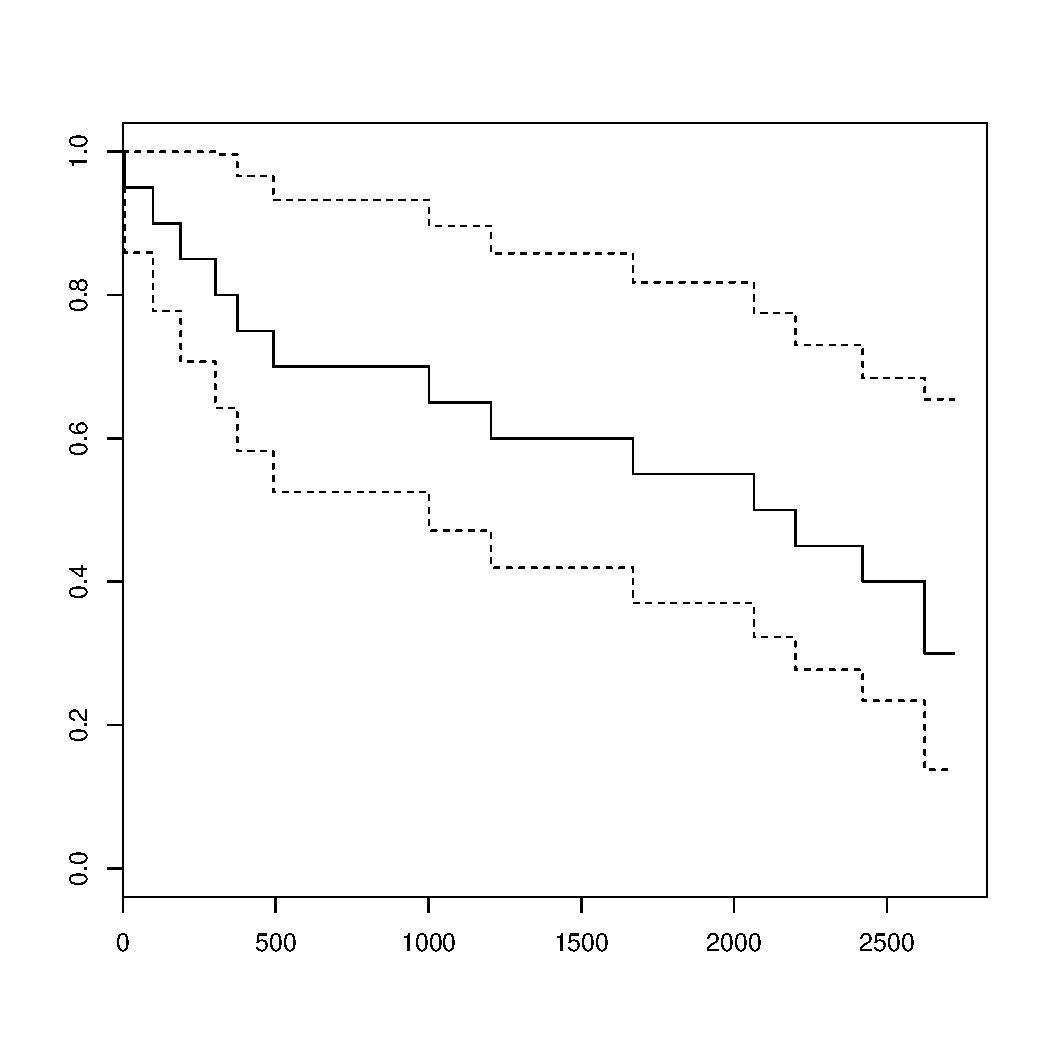
\includegraphics[scale = .28]{km1}\hspace{.2cm}
    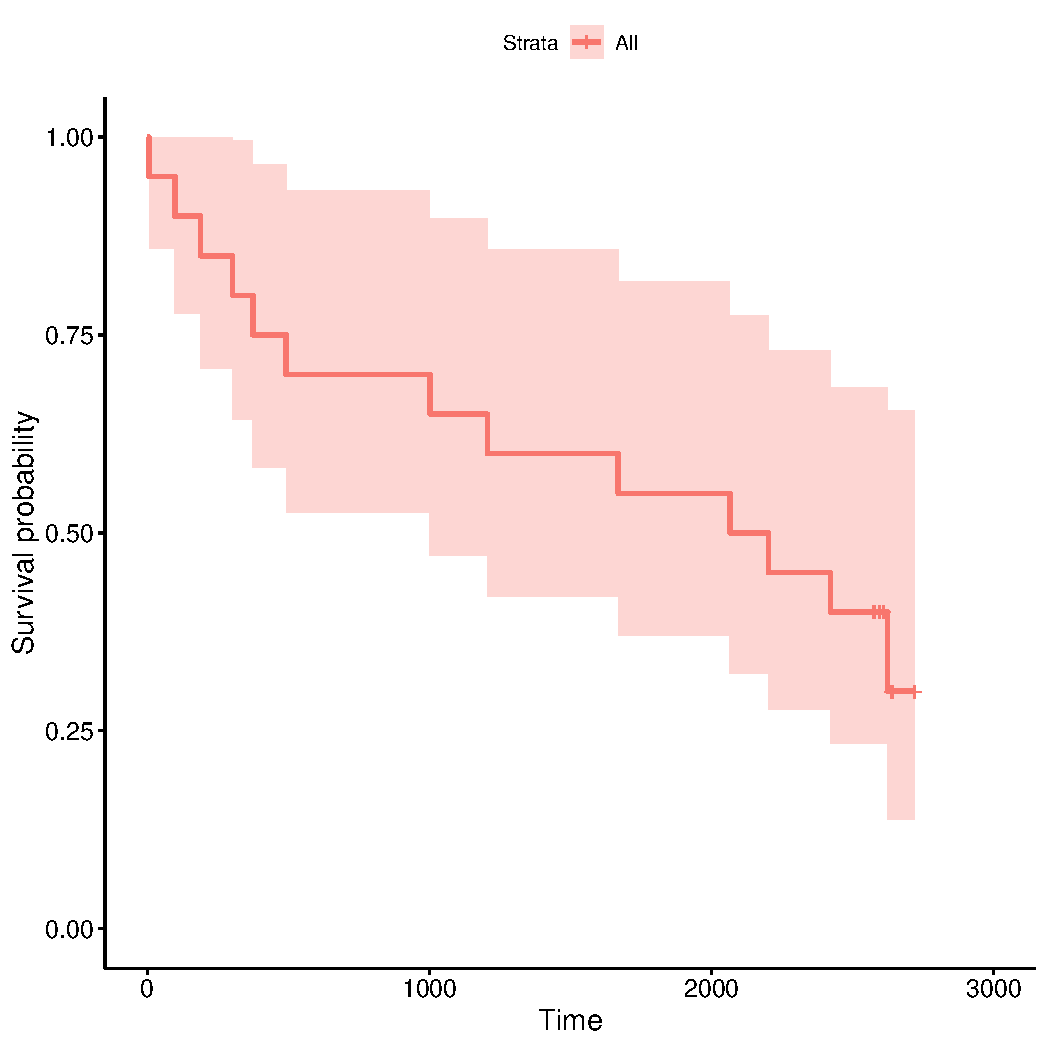
\includegraphics[scale = .28]{km2}
  \item Since \pkg{survminer} depends on the newest version of \pkg{survMisc},
    you might need to update the latter to be able to use \code{ggsurvplot}.
  \end{itemize}
\end{frame}

\begin{frame}
  \frametitle{Kaplan-Meier estimator}
  Suppose we want $\p(T > 800)$ based on the following modified data:
  \begin{columns}
    \column{0.45\textwidth}
    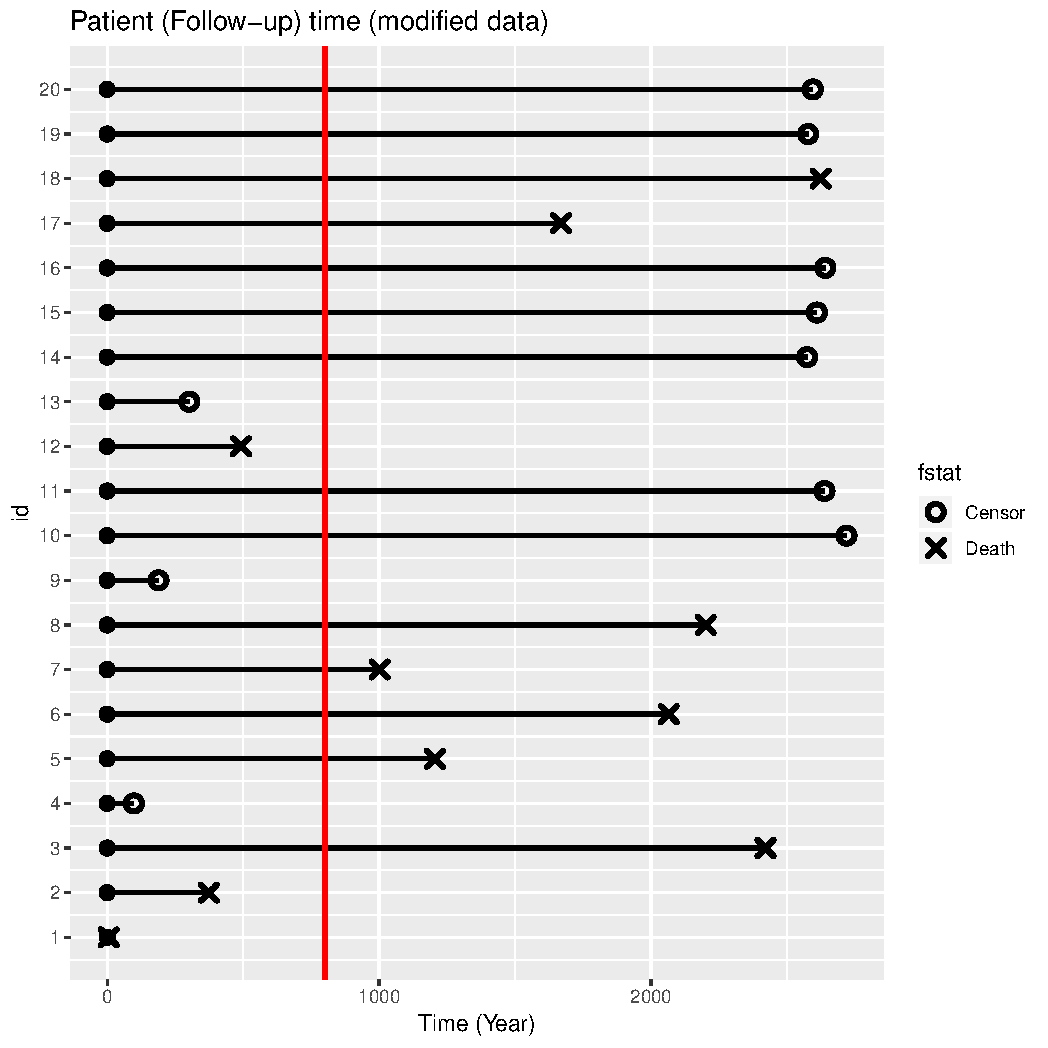
\includegraphics[scale = .3]{tab1-1-5}
    \column{0.55\textwidth}
    \begin{itemize}
    \item There are 3 events before $t = 800$.
    \item The events occured at 
      {\scriptsize
      \begin{tabular}{lllllll}
        $t_{(0)}$ & $t_{(1)}$ & $t_{(2)}$ & $t_{(3)}$ \\
        \midrule
        0 & 6 & 374 & 492 \\
      \end{tabular}}
    \item In this modified data, $t = 98, 189, 302$ are considered as censored.
    \end{itemize}
  \end{columns}
  \vspace{-.3cm}
  {\scriptsize
  \begin{align*}
    \Skm(800) &= \p(T > 800) =\\
    &= \p(T > 0) \times \p(T > 6|T > 0) \times \p(T > 374|T > 6) \times \p(T > 492|T > 374) \\
    &=1 \times \frac{19}{20} \times \frac{15}{16} \times \frac{14}{15} \approx 83.1\%
  \end{align*}
  }
\end{frame}

\begin{frame}[fragile]
  \frametitle{Kaplan-Meier estimator}
  \begin{itemize}
  \item The Kaplan-Meier estimator for the whole data is
\begin{knitrout}\scriptsize
\definecolor{shadecolor}{rgb}{0.969, 0.969, 0.969}\color{fgcolor}\begin{kframe}
\begin{alltt}
\hlstd{> }\hlkwd{library}\hlstd{(survival)}
\hlstd{> }\hlstd{km} \hlkwb{<-} \hlkwd{survfit}\hlstd{(}\hlkwd{Surv}\hlstd{(lenfol, fstat)} \hlopt{~} \hlnum{1}\hlstd{,} \hlkwc{data} \hlstd{= whas100)}
\hlstd{> }\hlkwd{plot}\hlstd{(km)}
\hlstd{> }\hlkwd{ggsurvplot}\hlstd{(km)}
\end{alltt}
\end{kframe}
\end{knitrout}
    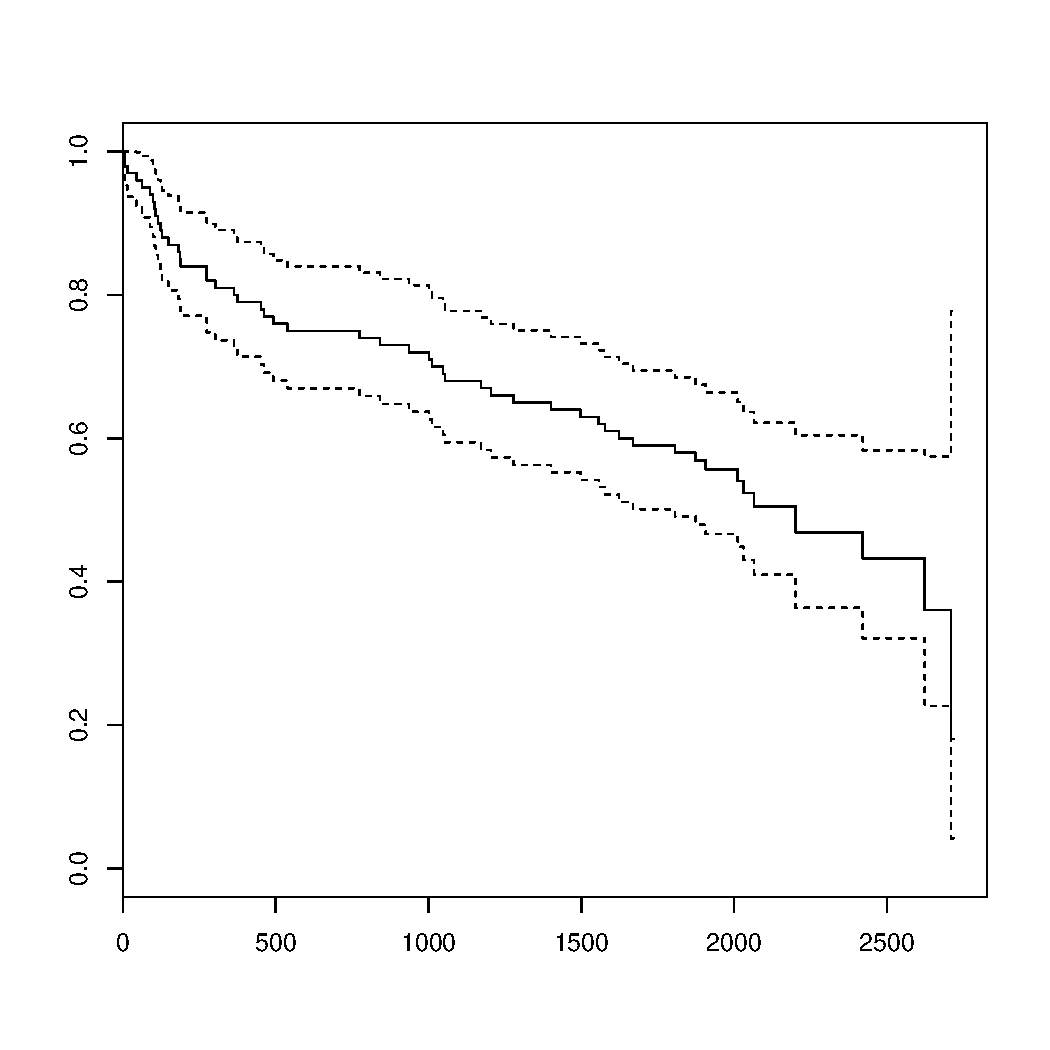
\includegraphics[scale = .28]{km3}\hspace{.2cm}
    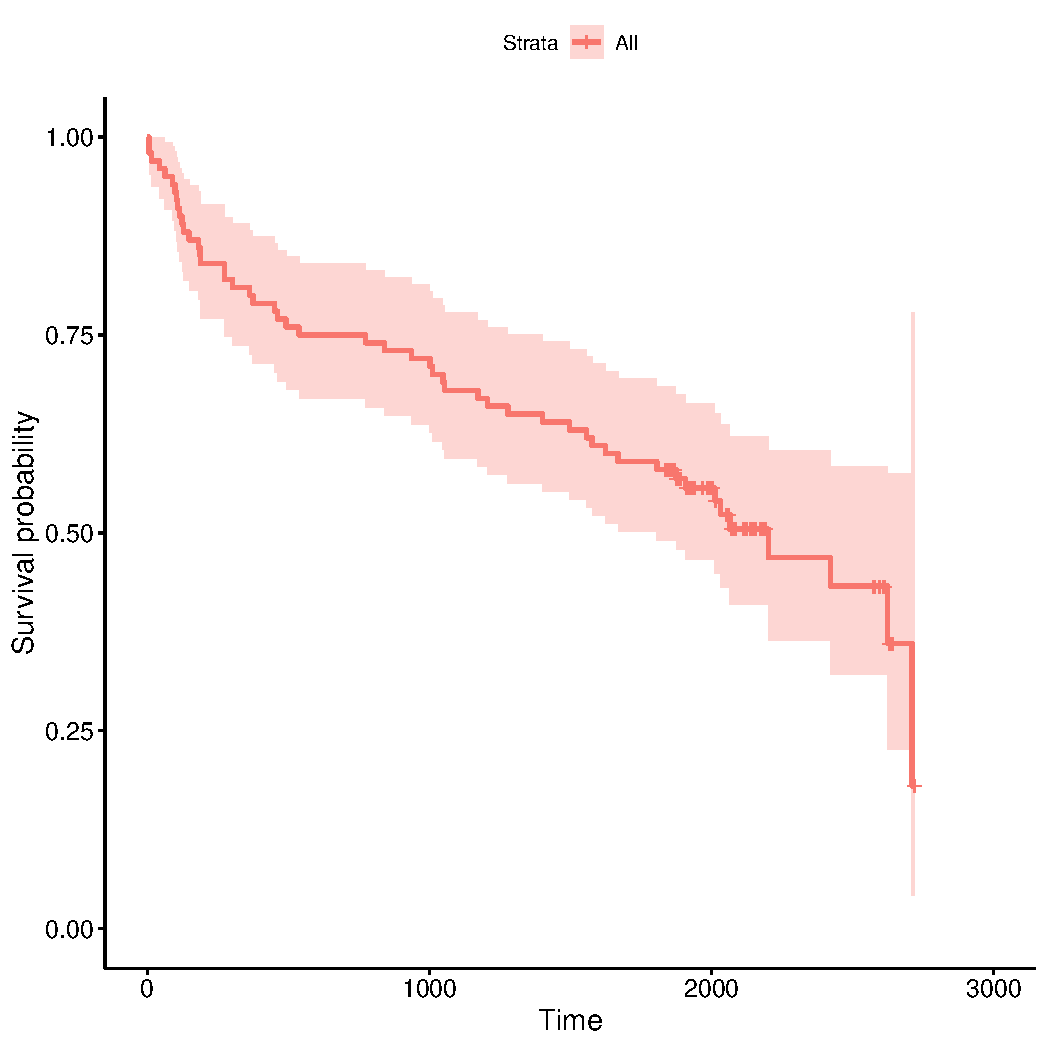
\includegraphics[scale = .28]{km4}
  \item If the last observed time corresponds to a censored observation, 
    then the estimate of the survival function does not go to zero.
  \end{itemize}    
\end{frame}


\begin{frame}
  \frametitle{Kaplan-Meier estimator}
  \begin{itemize}
  \item Suppose we have a sample of $n$ independent observations $(t_i, c_i), i = 1, 2, \ldots, n$.
  \item There are $m$ deaths and $m\le n$.
  \item The series $\{t_{(1)}, \ldots, t_{(m)}\}$ are the $m$ ordered death times.
  \item The Kaplan-Meier estimator has the form
    \begin{equation*}
      \Skm(t) = \sum_{t_{(i)} \le t}\frac{n_i - d_i}{n_i} = \sum_{t_{(i)} \le t} 1 - \frac{d_i}{n_i},
    \end{equation*}
    where $n_i$ is the number of individual who are alive at $t_{(i)}$ (at risk),
    and $d_i$ is the number of individual who died at $t_{(i)}$.
  \item A potential problem with the Kaplan-Meier estimator is when $n_i$ is small and
    $n_i = d_i$ occurs at early time.
  \end{itemize}    
\end{frame}

\begin{frame}
  \frametitle{Nelson-Aalon estimator}
  \begin{itemize}
  \item An alternative estimate of $\Skm(t)$ is the \empr{Nelson-Aalon estimator}:
    \begin{equation*}
      \Sna(t) = \prod_{t_{(i)} \le t} \exp\left(-\frac{d_i}{n_i}\right).
    \end{equation*}
  \item The main idea is to see $d_i/n_i$ as the event rate, i.e., $h(t_{(i)}) = d_i/n_i$.
  \item Recall the relationship $h(t) = f(t) / S(t)$ and think of $d_i/n$ and $n_i/n$ 
    are raw rough estimates of $f(t)$ and $S(t)$.
  \item By the similar argument, we have
    $$H(t) = \sum_{t_{(i)} \le t} d_i/n_i, \mbox{ and } S(t) = e^{-H(t)} = \Sna(t).$$
  \item $\Sna(t)$ and $\Skm(t)$ are derived differently, but both based on $d_i$ and $n_i$.
  \item In general $\Sna(t)\neq\Skm(t)$ but $\Sna(t)\approx\Skm(t)$.
  \item $\Sna(t)$ has slightly nicer properties and is more stable.
  \end{itemize}
\end{frame}


\begin{frame}[fragile]
  \frametitle{Nelson-Aalon estimator}
  \begin{itemize}
  \item
  \end{itemize}
\end{frame}

\end{document}


